% Scalable Heteroscedastic GP: architecture flowchart + critical novelty review.
% Standalone Overleaf document (companion to heteroscedastic_nigp_combined.tex).
%
% Compile: pdfLaTeX -> BibTeX -> pdfLaTeX -> pdfLaTeX
% Self-contained in notes/: use \bibliography{hetero_nigp} (this file).
% Or set project root to Final_Report_JPL/ and switch to \bibliography{ref}.
%
% Diagram layout rules used here (avoid overlap):
%   - one figure environment per graphic; \FloatBarrier between figures
%   - fixed text widths + generous node distance
%   - orthogonal / vertical edges only; no crossing diagonals where possible
%   - never place two tikzpictures in the same float
\documentclass[11pt]{article}

\usepackage[margin=1in]{geometry}
\usepackage{amsmath,amssymb,mathtools}
\usepackage{booktabs}
\usepackage{tabularx}
\usepackage{array}
\usepackage{graphicx}
\usepackage{hyperref}
\usepackage{xcolor}
\usepackage{caption}
\usepackage{enumitem}
\usepackage{placeins}
\usepackage{float}
\usepackage{tikz}
\usepackage{natbib}
\usetikzlibrary{arrows.meta,positioning,fit,calc,shapes.geometric}

\hypersetup{colorlinks=true, linkcolor=blue!55!black, urlcolor=blue!55!black,
  citecolor=blue!55!black}

\renewcommand{\arraystretch}{1.35}
\setlength{\tabcolsep}{6pt}
\captionsetup{skip=10pt, font=small}
\setlength{\textfloatsep}{20pt plus 4pt minus 4pt}
\setlength{\floatsep}{18pt plus 4pt minus 2pt}
\setlength{\intextsep}{18pt plus 4pt minus 2pt}

% Shared TikZ styles (non-overlapping boxes)
\tikzset{
  >={Stealth[length=2.2mm]},
  every picture/.style={font=\scriptsize},
  box/.style={
    draw=black!70, rounded corners=2pt, align=center,
    inner sep=4pt, outer sep=1pt,
    minimum height=9mm,
    fill=white
  },
  boxentry/.style={box, text width=3.6cm, fill=blue!6},
  boxmodel/.style={box, text width=2.7cm, fill=gray!8},
  boxctrl/.style={box, text width=2.9cm, fill=orange!10},
  boxtrain/.style={box, text width=3.2cm, fill=green!8},
  boxpred/.style={box, text width=3.0cm, fill=teal!12},
  boxphase/.style={box, text width=3.4cm, minimum height=18mm, fill=white},
  arr/.style={->, thick, draw=black!60},
  lab/.style={font=\scriptsize\itshape, text=black!55},
  group/.style={draw=black!35, dashed, rounded corners=3pt, inner sep=6pt},
}

\newcommand{\sigy}{\sigma_{y}^{2}}
\newcommand{\sigyhom}{\sigma_{y,\mathrm{hom}}^{2}}
\newcommand{\sighet}{\sigma_{y,\mathrm{het}}^{2}}
\newcommand{\signigp}{\sigma_{\mathrm{nigp}}^{2}}
\newcommand{\sigeff}{\sigma_{\mathrm{eff}}^{2}}
\newcommand{\sigobs}{\sigma_{y|\mathcal{D}}^{2}}
\newcommand{\Sigx}{\Sigma_{x}}
\newcommand{\Phif}{\Phi_{f}}
\newcommand{\Cy}{C_{y}}

\title{Scalable Heteroscedastic GP:\\[0.25em]
\large Architecture Flowchart and Critical Novelty Review}
\author{SpectralGPPlus --- Additive Residual Hetero-NIGP (S5)\\
\small Companion critique to \texttt{heteroscedastic\_nigp\_combined}}
\date{}

\begin{document}
\maketitle

\begin{abstract}
\noindent
This note documents the \textbf{code-mapped} path for Additive Residual
Hetero-NIGP in SpectralGPPlus (experiment S5), states the core equations,
and gives a critical novelty assessment.
The single-task stack is a domain-motivated composition of known pieces
(heteroscedastic nugget + McHutchon NIGP + SORF/Woodbury), not a new GP theory.
A separate section reviews multitask ICM-SORF with NIGP and the
\emph{unimplemented} extension to heteroscedastic Noise SORF.
TikZ diagrams are laid out one-per-float with fixed box widths and large
vertical spacing so graphics do not overlap.
\end{abstract}

\paragraph{Novelty verdict (short).}
No strong claim of new GP theory is warranted.
Accurate label: \emph{scalable, instrument-aware hetero$+$NIGP for spectral
retrieval} --- not a ``novel heteroscedastic GP.''
The multitask $\times$ NIGP $\times$ Noise-SORF \emph{triple} is
\textbf{not implemented}; free Noise SORF exists only on single-task
\texttt{RFFGPR} (S5).

\FloatBarrier
\section{Architecture flowchart (single-task S5)}
\label{sec:arch}

Hot path:
\texttt{S5\_emit\_heteroscedastic\_SORF.py}
$\to$
\texttt{emit\_s4\_sorf\_base.run\_s4\_emit\_sorf}
$\to$
\texttt{RFFGPR(hetero\_sorf=True)}
with Noise SORF + NIGP flags
$\to$ Woodbury on $\Cy=\mathrm{diag}(\sigeff)+\Phif\Phif^{\top}$.
There is \emph{no} dedicated heteroscedastic likelihood class; hetero layers on
\texttt{LogGaussianLikelihood} (scalar $\sigyhom$) plus
\texttt{NoiseSORFLogNoise}.

% Absolute coordinates (cm grid). Row/column gaps keep boxes from overlapping.
% One tikzpicture per float; \FloatBarrier between figures.

\begin{figure}[H]
\centering
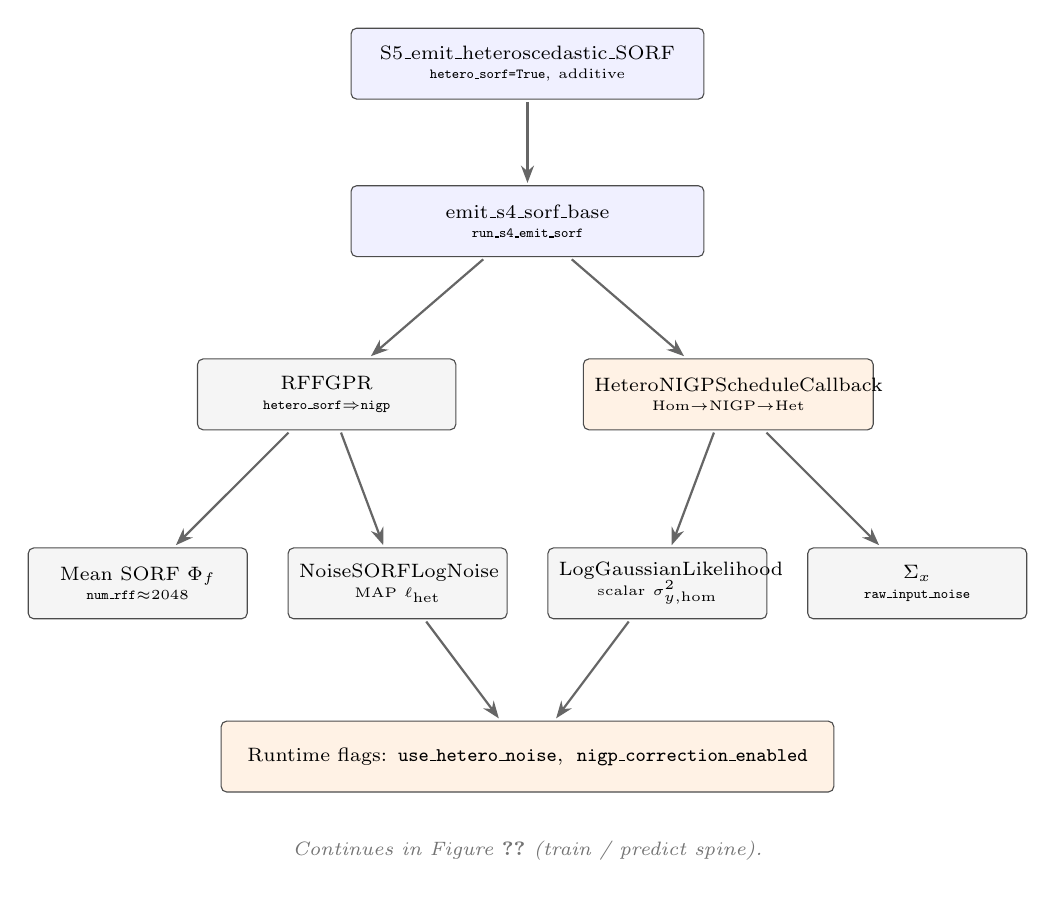
\begin{tikzpicture}
  % Columns x = 0, 3.3, 6.6, 9.9 ; rows y = 0, -2.4, -4.8, -7.2
  \node[boxentry, text width=4.2cm] (s5) at (4.95, 0.0)
    {S5\_emit\_heteroscedastic\_SORF\\[-1pt]
     {\tiny\texttt{hetero\_sorf=True}, additive}};
  \node[boxentry, text width=4.2cm] (base) at (4.95, -2.0)
    {emit\_s4\_sorf\_base\\[-1pt]{\tiny\texttt{run\_s4\_emit\_sorf}}};

  \node[boxmodel, text width=3.0cm] (model) at (2.4, -4.2)
    {RFFGPR\\[-1pt]{\tiny\texttt{hetero\_sorf}$\Rightarrow$\texttt{nigp}}};
  \node[boxctrl, text width=3.4cm] (sched) at (7.5, -4.2)
    {HeteroNIGPScheduleCallback\\[-1pt]{\tiny Hom$\to$NIGP$\to$Het}};

  \node[boxmodel, text width=2.5cm] (mean) at (0.0, -6.6)
    {Mean SORF $\Phif$\\[-1pt]{\tiny\texttt{num\_rff}$\approx$2048}};
  \node[boxmodel, text width=2.5cm] (noise) at (3.3, -6.6)
    {NoiseSORFLogNoise\\[-1pt]{\tiny MAP $\ell_{\mathrm{het}}$}};
  \node[boxmodel, text width=2.5cm] (lik) at (6.6, -6.6)
    {LogGaussianLikelihood\\[-1pt]{\tiny scalar $\sigyhom$}};
  \node[boxmodel, text width=2.5cm] (sigx) at (9.9, -6.6)
    {$\Sigx$\\[-1pt]{\tiny\texttt{raw\_input\_noise}}};

  \node[boxctrl, text width=7.5cm] (flags) at (4.95, -8.8)
    {Runtime flags:
     \texttt{use\_hetero\_noise},\;
     \texttt{nigp\_correction\_enabled}};

  \draw[arr] (s5) -- (base);
  \draw[arr] (base) -- (model);
  \draw[arr] (base) -- (sched);
  \draw[arr] (model) -- (mean);
  \draw[arr] (model) -- (noise);
  \draw[arr] (sched) -- (lik);
  \draw[arr] (sched) -- (sigx);
  \draw[arr] (noise) -- (flags);
  \draw[arr] (lik) -- (flags);

  \node[lab] at (4.95, -10.0)
    {Continues in Figure~\ref{fig:arch-train} (train / predict spine).};
\end{tikzpicture}
\caption{S5 construction path: experiment entry, model pieces, and schedule flags.
Absolute grid spacing ($\Delta x=3.3$\,cm, $\Delta y\ge 2$\,cm) prevents overlap.}
\label{fig:arch-build}
\end{figure}

\FloatBarrier

\begin{figure}[H]
\centering
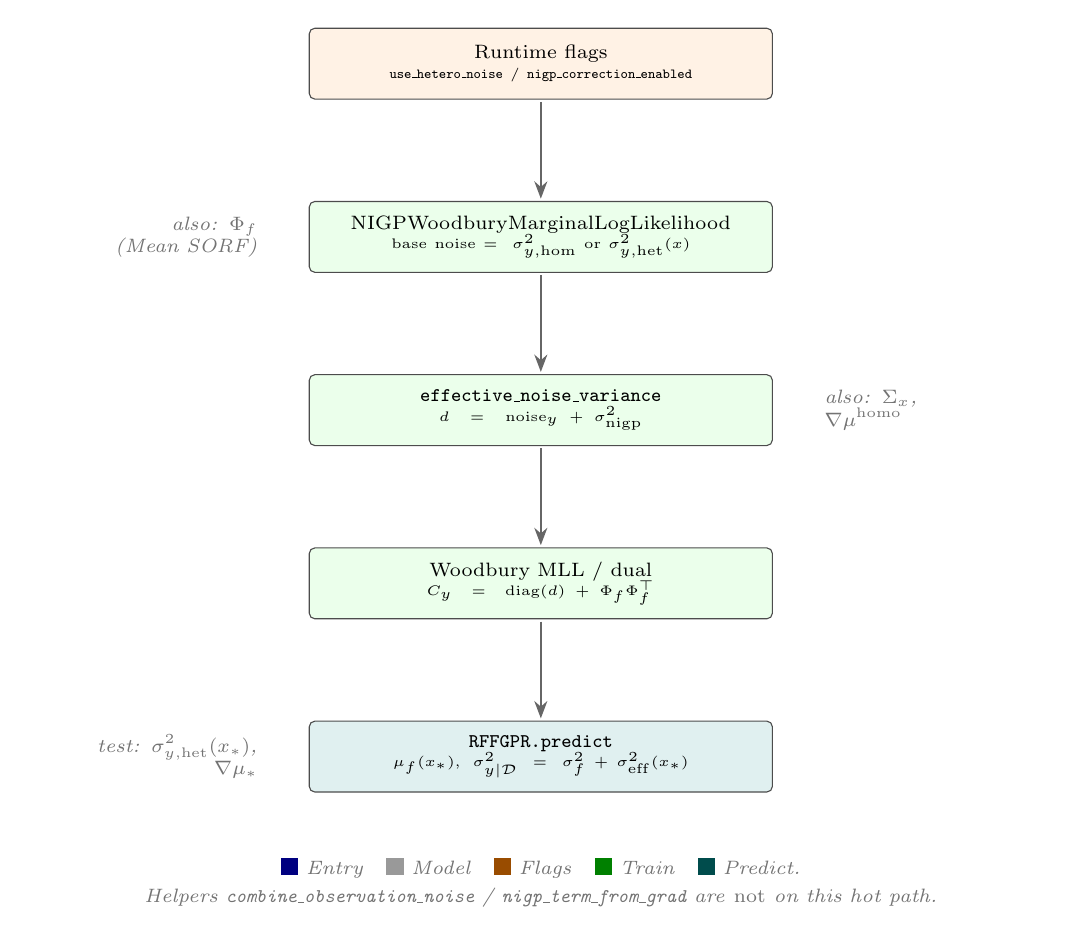
\begin{tikzpicture}
  % Single centered column; side notes outside the 3.6cm box width
  \node[boxctrl, text width=5.6cm] (flags) at (0, 0.0)
    {Runtime flags\\[-1pt]
     {\tiny\texttt{use\_hetero\_noise} / \texttt{nigp\_correction\_enabled}}};
  \node[boxtrain, text width=5.6cm] (mll) at (0, -2.2)
    {NIGPWoodburyMarginalLogLikelihood\\[-1pt]
     {\tiny base noise $=\sigyhom$ or $\sighet(x)$}};
  \node[boxtrain, text width=5.6cm] (eff) at (0, -4.4)
    {\texttt{effective\_noise\_variance}\\[-1pt]
     {\tiny $d=\mathrm{noise}_y+\signigp$}};
  \node[boxtrain, text width=5.6cm] (wb) at (0, -6.6)
    {Woodbury MLL / dual\\[-1pt]
     {\tiny $\Cy=\mathrm{diag}(d)+\Phif\Phif^{\top}$}};
  \node[boxpred, text width=5.6cm] (pred) at (0, -8.8)
    {\texttt{RFFGPR.predict}\\[-1pt]
     {\tiny $\mu_f(x_{*})$,\;
      $\sigobs=\sigma_f^{2}+\sigeff(x_{*})$}};

  \draw[arr] (flags) -- (mll);
  \draw[arr] (mll) -- (eff);
  \draw[arr] (eff) -- (wb);
  \draw[arr] (wb) -- (pred);

  \node[lab, text width=2.8cm, align=right] at (-5.0, -2.2)
    {also: $\Phif$\\(Mean SORF)};
  \node[lab, text width=2.8cm, align=left] at (5.0, -4.4)
    {also: $\Sigx$,\\$\nabla\mu^{\mathrm{homo}}$};
  \node[lab, text width=2.8cm, align=right] at (-5.0, -8.8)
    {test: $\sighet(x_{*})$,\\$\nabla\mu_{*}$};

  \node[lab, text width=12cm, align=center] at (0, -10.4)
    {\textcolor{blue!50!black}{\rule{2.2mm}{2.2mm}}~Entry\quad
     \textcolor{black!40}{\rule{2.2mm}{2.2mm}}~Model\quad
     \textcolor{orange!60!black}{\rule{2.2mm}{2.2mm}}~Flags\quad
     \textcolor{green!50!black}{\rule{2.2mm}{2.2mm}}~Train\quad
     \textcolor{teal!60!black}{\rule{2.2mm}{2.2mm}}~Predict.\\[2pt]
     Helpers \texttt{combine\_observation\_noise} /
     \texttt{nigp\_term\_from\_grad} are \emph{not} on this hot path.};
\end{tikzpicture}
\caption{S5 train/predict spine (continuation of Figure~\ref{fig:arch-build}).
Pure vertical column; side notes sit outside the boxes.}
\label{fig:arch-train}
\end{figure}

\FloatBarrier
\section{Core equations}
\label{sec:eq}

\paragraph{Additive Residual Hetero-NIGP (H3).}
\begin{equation}
  \sigeff(x)
  \;=\;
  \sighet(x)
  \;+\;
  \signigp(x),
  \qquad
  \signigp(x)
  \;=\;
  \sum_{k}\sigma_{x,k}^{2}\,
  \bigl(\partial_{x_k}\mu^{\mathrm{homo}}(x)\bigr)^{2}.
\end{equation}
The Jacobian $\nabla\mu$ comes from a \textbf{homoskedastic} dual solve and is
\textbf{detached}.
Slopes always use scalar \texttt{likelihood.noise}, even after hetero unlock.

\paragraph{Noise SORF (S5 v1 MAP).}
\begin{equation}
  \ell_{\mathrm{het}}(x)=b+w^{\top}\phi_{\mathrm{het}}(x),
  \qquad
  \sighet(x)=10^{\mathrm{SoftClamp}(\ell_{\mathrm{het}}(x))}.
\end{equation}
Only the MAP mean of $\ell_{\mathrm{het}}$ enters $\sigeff$; predictive variance
of the noise field is discarded.

\paragraph{Woodbury and prediction.}
\begin{equation}
  \Cy=\mathrm{diag}(d)+\Phif\Phif^{\top},
  \qquad
  \mu_{y}(x_{*})=\mu_{f}(x_{*}),
  \qquad
  \sigobs(x_{*})=\sigma_{f}^{2}(x_{*})+\sigeff(x_{*}).
\end{equation}

\FloatBarrier
\section{Training phase schedule}
\label{sec:schedule}

Defaults in \texttt{S5\_emit\_heteroscedastic\_SORF.py}:
\texttt{EPOCHS\_HOM$=$200}, \texttt{EPOCHS\_HET$=$1}, \texttt{NUM\_EPOCHS$=$1000}.
The dedicated NIGP-only window is therefore \textbf{one epoch}.
Slope refreshes occur at NIGP unlock and at the last epoch only.

\begin{figure}[H]
\centering
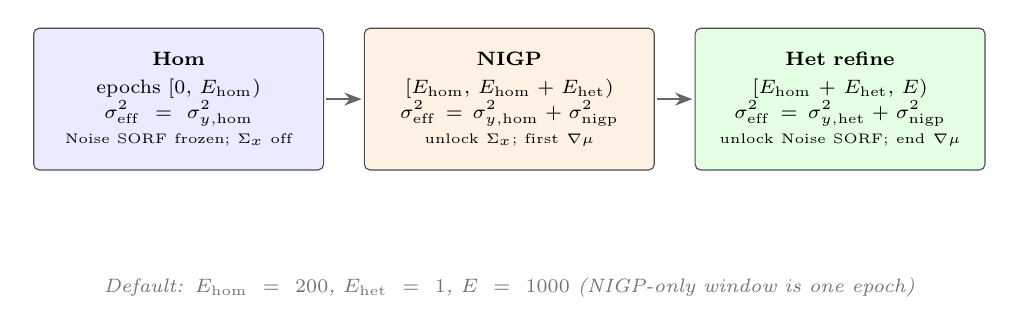
\begin{tikzpicture}
  % Three phase boxes on one row; centers 4.2cm apart (text width 3.4cm + gap)
  \node[boxphase, fill=blue!8] (hom) at (0.0, 0.0) {%
    \textbf{Hom}\\[2pt]
    epochs $[0,\,E_{\mathrm{hom}})$\\[1pt]
    $\sigeff=\sigyhom$\\[1pt]
    {\tiny Noise SORF frozen; $\Sigx$ off}};
  \node[boxphase, fill=orange!10] (nigp) at (4.2, 0.0) {%
    \textbf{NIGP}\\[2pt]
    $[E_{\mathrm{hom}},\,E_{\mathrm{hom}}+E_{\mathrm{het}})$\\[1pt]
    $\sigeff=\sigyhom+\signigp$\\[1pt]
    {\tiny unlock $\Sigx$; first $\nabla\mu$}};
  \node[boxphase, fill=green!10] (het) at (8.4, 0.0) {%
    \textbf{Het refine}\\[2pt]
    $[E_{\mathrm{hom}}+E_{\mathrm{het}},\,E)$\\[1pt]
    $\sigeff=\sighet+\signigp$\\[1pt]
    {\tiny unlock Noise SORF; end $\nabla\mu$}};

  \draw[arr] (hom) -- (nigp);
  \draw[arr] (nigp) -- (het);

  \node[lab, text width=12cm, align=center] at (4.2, -2.4)
    {Default: $E_{\mathrm{hom}}=200$, $E_{\mathrm{het}}=1$, $E=1000$
     (NIGP-only window is one epoch)};
\end{tikzpicture}
\caption{S5 three-phase Adam schedule
(\texttt{HeteroNIGPScheduleCallback}).
With $E_{\mathrm{het}}=1$, free Noise SORF unlocks almost immediately after
NIGP---risk that $\sighet$ absorbs variance intended for $\signigp$.}
\label{fig:schedule}
\end{figure}

\begin{table}[H]
\centering
\small
\begin{tabular}{@{}>{\raggedright\arraybackslash}p{1.6cm}
  >{\raggedright\arraybackslash}p{2.2cm}
  >{\raggedright\arraybackslash}p{3.0cm}
  >{\raggedright\arraybackslash}p{4.2cm}
  >{\raggedright\arraybackslash}p{2.6cm}@{}}
\toprule
\textbf{Phase} & \textbf{Epochs (default)} & $\sigeff$ &
\textbf{Trainable noise} & \textbf{NIGP / slopes} \\
\midrule
Hom & $[0,200)$ & $\sigyhom$ &
\texttt{raw\_noise} on; Noise SORF / $\Sigx$ frozen & off \\
NIGP & $[200,201)$ & $\sigyhom+\signigp$ &
freeze \texttt{raw\_noise}+Noise SORF; unlock $\Sigx$ & first $\nabla\mu$ \\
Het & $[201,1000)$ & $\sighet+\signigp$ &
Noise SORF warm-started + unlocked; $\Sigx$ on & endpoint $\nabla\mu$ \\
\bottomrule
\end{tabular}
\caption{Phase table matching Figure~\ref{fig:schedule}.}
\label{tab:phases}
\end{table}

\FloatBarrier
\section{Model ladder (H0--H3)}
\label{sec:ladder}

\begin{table}[H]
\centering
\small
\begin{tabular}{@{}lllll@{}}
\toprule
\textbf{ID} & \textbf{Model} & $\Sigx$ / NIGP & $\sighet(x)$ & \textbf{Status} \\
\midrule
H0 & Homoscedastic SORF & off & $\equiv\sigy$ & Implemented (base) \\
H1 & NIGP-only & learn & $\equiv\sigy$ & S4 / \texttt{main.tex} \\
H2 & Hetero-only & off & free (Noise SORF) & Code path via flags \\
H3 & Additive Residual Hetero-NIGP & learn & free (Noise SORF) & S5 v1 \\
\bottomrule
\end{tabular}
\caption{Ablation ladder from the design notes.
Success criterion (not yet closed in \texttt{main.tex}): H3 improves
calibration vs.\ H1 without hurting RRMSE; $\sighet$ and $\signigp$ are not
redundant.}
\label{tab:ladder}
\end{table}

\FloatBarrier
\section{Novelty scorecard (single-task)}
\label{sec:novelty}

\begin{table}[H]
\centering
\small
\begin{tabular}{@{}>{\raggedright\arraybackslash}p{3.6cm}
  >{\raggedright\arraybackslash}p{4.0cm}
  >{\raggedright\arraybackslash}p{4.0cm}@{}}
\toprule
\textbf{Prior art (not invented here)} &
\textbf{Defensible contribution} &
\textbf{Overclaim risk} \\
\midrule
Heteroscedastic GPs
\cite{goldberg1998heteroscedastic,kersting2007mlhgp,lazaro2011vhgp}
& Domain split: instrument $\Sigx$ vs.\ RT/scene residual hetero
& \texttt{main.tex} still reports SORF$+$NIGP only \\[0.4em]
NIGP linearization \cite{mchutchon2011nigp}
& Scalable MAP Noise SORF ($D_{\mathrm{het}}\ll D_f$) on Woodbury diagonal
& H0--H3 framed as follow-on; utility novelty unproven \\[0.4em]
RFF/ORF/SORF $+$ Woodbury
\cite{rahimi2007rff,yu2016orf,cutajar2017dgp}
& Hom $\to$ NIGP $\to$ Het unlock $+$ warm-start $+$ sparse slope cache
& MAP plug-in $\neq$ Goldberg/VHGP noise posterior \\[0.4em]
Adding two positive diagonal noise sources
& --- & --- \\
\bottomrule
\end{tabular}
\caption{Novelty scorecard for single-task Additive Residual Hetero-NIGP.}
\label{tab:novelty}
\end{table}

\paragraph{What is not novel.}
Heteroscedastic likelihoods; NIGP two-step slopes; RFF/SORF$+$Woodbury scalability;
adding two positive diagonal noise sources.

\paragraph{Talk line (from the design notes).}
NIGP explains input-driven $\signigp$; free $\sighet(x)$ explains residual
scene-dependent output noise that slopes cannot---add them as
$\sigeff=\sighet+\signigp$ on the diagonal and keep the same Woodbury path.
Fair engineering summary; do not inflate into new GP theory without H1/H2/H3
evidence.

\FloatBarrier
\section{Critical failure modes (single-task)}
\label{sec:risks}

\begin{table}[H]
\centering
\small
\begin{tabular}{@{}>{\raggedright\arraybackslash}p{2.4cm}
  >{\raggedright\arraybackslash}p{4.6cm}
  >{\raggedright\arraybackslash}p{4.6cm}@{}}
\toprule
\textbf{Risk} & \textbf{Why it matters} & \textbf{Mitigation / status} \\
\midrule
Identifiability
& $\sighet$ and $\signigp$ both inflate $\mathrm{diag}(\Cy)$
& Phased unlock; SoftClamp; NEDL-anchored $\Sigx$ still an idea \\
MAP noise, discarded var
& Uncertainty about $\ell_{\mathrm{het}}$ never enters $\sigeff$
& Documented v1 choice; full second GP unused \\
Stacked NIGP approx
& Homo dual slopes, detached $\nabla\mu$, only two refreshes
& Matches McHutchon spirit; not joint each step \\
Schedule fragility
& $E_{\mathrm{het}}=1$ barely exercises NIGP-only before hetero unlock
& Tune epochs; ablate H1/H2/H3 \\
Slope asymmetry
& $\nabla\mu$ always from scalar \texttt{likelihood.noise}
& By design (frozen dual); inconsistent with joint hetero \\
Evidence gap
& Unit tests cover schedule mechanics, not scientific success
& Need RRMSE $+$ NIS/ASD coverage vs.\ H1 \\
Unimplemented ideas
& Multiplicative combine; hetero MT; noise-GP variance; NEDL $\Sigx$
& Documented only --- not delivered capability \\
\bottomrule
\end{tabular}
\caption{Single-task methodological risks.}
\label{tab:risks}
\end{table}

\FloatBarrier
\section{Critical review: multitask GP + NIGP + hetero Noise SORF}
\label{sec:mt}

\subsection{Status of the triple stack}

Do \textbf{not} treat MT $\times$ NIGP $\times$ heteroscedastic Noise SORF as a
delivered model.
What exists is multitask ICM-SORF with classic NIGP
(\texttt{RFFMTGPR} $+$ \texttt{NIGPMTWoodburyMarginalLogLikelihood}).
Free Noise SORF lives only on single-task \texttt{RFFGPR} (S5).
QoI-coupled multitask noise (ICM on $\ell_{\mathrm{het},t}$) is design-note
idea~\#5 only; the notes themselves say do independent per-QoI $\sighet,t$ first.

\begin{figure}[H]
\centering
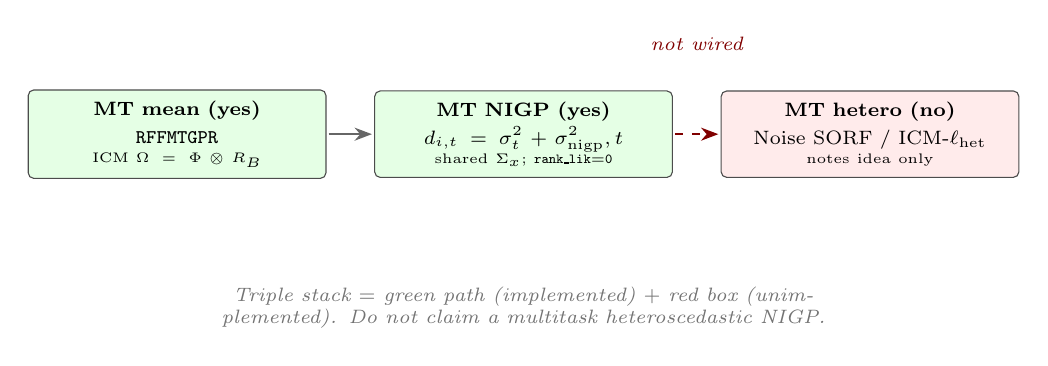
\begin{tikzpicture}
  \node[boxmodel, text width=3.5cm, fill=green!10] (mtmean) at (0.0, 0.0)
    {\textbf{MT mean (yes)}\\[2pt]
     \texttt{RFFMTGPR}\\[-1pt]
     {\tiny ICM $\Omega=\Phi\otimes R_B$}};
  \node[boxmodel, text width=3.5cm, fill=green!10] (mtnigp) at (4.4, 0.0)
    {\textbf{MT NIGP (yes)}\\[2pt]
     $d_{i,t}=\sigma_{t}^{2}+\signigp,t$\\[-1pt]
     {\tiny shared $\Sigx$; \texttt{rank\_lik$=$0}}};
  \node[boxmodel, text width=3.5cm, fill=red!8] (mthet) at (8.8, 0.0)
    {\textbf{MT hetero (no)}\\[2pt]
     Noise SORF / ICM-$\ell_{\mathrm{het}}$\\[-1pt]
     {\tiny notes idea only}};

  \draw[arr] (mtmean) -- (mtnigp);
  \draw[arr, dashed, draw=red!50!black] (mtnigp) -- (mthet);
  \node[lab, text=red!50!black] at (6.6, 1.15) {not wired};

  \node[lab, text width=12cm, align=center] at (4.4, -2.2)
    {Triple stack $=$ green path (implemented) $+$ red box (unimplemented).
     Do not claim a multitask heteroscedastic NIGP.};
\end{tikzpicture}
\caption{Multitask capability split.
Implemented pieces are left/center; heteroscedastic Noise SORF on MT is absent.}
\label{fig:mt-status}
\end{figure}

\begin{table}[H]
\centering
\small
\begin{tabular}{@{}>{\raggedright\arraybackslash}p{4.0cm}
  >{\raggedright\arraybackslash}p{4.2cm}
  >{\raggedright\arraybackslash}p{4.2cm}@{}}
\toprule
\textbf{Capability} & \textbf{Single-task (S4/S5)} & \textbf{Multitask (MTGPR)} \\
\midrule
Mean SORF/RFF $+$ Woodbury
& \texttt{RFFGPR}
& \texttt{RFFMTGPR} (ICM) \\
Classic NIGP (scalar output noise $+$ $\Sigx$)
& Implemented (S4)
& Implemented (\texttt{nigp\_mt\_mll}) \\
Free Noise SORF $\sighet(x)$
& Implemented (S5 v1 MAP)
& \textbf{Not present} on \texttt{RFFMTGPR} \\
Additive $\sigeff=\sighet+\signigp$
& S5 schedule $+$ flags
& Not wired \\
\texttt{HeteroNIGPScheduleCallback}
& Yes
& No MT analogue \\
ICM / shared $\ell_{\mathrm{het}}$ across QoIs
& N/A
& Documented idea only \\
\bottomrule
\end{tabular}
\caption{ST vs.\ MT capability matrix.}
\label{tab:mt-cap}
\end{table}

\subsection{What MT + NIGP actually implements}

\begin{itemize}[leftmargin=1.2em,itemsep=0.35em]
  \item \textbf{Mean:} spatial features $\Phi$ and ICM factor $R_B$ give
        $\Omega=\Phi\otimes R_B$; joint Woodbury on flattened $(n\cdot T)$ targets
        (\texttt{experiments\_RFFMTGPR/emit\_s4\_mtgpr\_runner.py}).
  \item \textbf{NIGP:}
        $d_{i,t}=\sigma_{t}^{2}+\sum_{d}\sigma_{x,d}^{2}(\partial_{d}\mu_{t}(x_{i}))^{2}$
        via \texttt{effective\_noise\_variance\_mt}; shared $\Sigx$; slopes from
        homoskedastic MT dual (\texttt{posterior\_mean\_grad\_wrt\_x\_mt}), detached.
  \item \textbf{Constraint:} \texttt{rank\_likelihood$=$0} --- no residual
        task-noise correlations in the likelihood when NIGP is on.
\end{itemize}

\subsection{Critiques of the proposed triple}

The design note imagines
$\sigeff,t(x)=\sighet,t(x)+\signigp,t(x)$
with optional ICM on $\ell_{\mathrm{het},t}$.
Scientifically motivated; statistically and engineering-wise this is the most
overfit-prone stacking in the repo.

\begin{table}[H]
\centering
\small
\begin{tabular}{@{}>{\raggedright\arraybackslash}p{3.2cm}
  >{\raggedright\arraybackslash}p{9.4cm}@{}}
\toprule
\textbf{Critique} & \textbf{Detail} \\
\midrule
Not a model --- a wishlist
& No \texttt{hetero\_sorf} on \texttt{RFFMTGPR}; no MT schedule; no S5-analogue entry.
Claiming a multitask heteroscedastic NIGP overstates code reality. \\
Identifiability cubed
& ICM mean correlations, shared $\Sigx$, and free (or ICM-coupled) hetero all
explain residuals. ST H3 already confounds $\sighet$ with $\signigp$; MT adds a
third channel. \\
Shared $\Sigx$ vs.\ task residual
& Instrument noise is shared (good story), but NIGP inflation is
task-dependent through $\nabla\mu_{t}$. Free hetero can silently take over
task-idiosyncratic residual. \\
Notes contradict premature ICM-on-noise
& Do independent per-QoI $\sighet,t$ before multitask noise (design note).
Jumping to ICM on $\ell_{\mathrm{het}}$ before ST H3 evidence is backwards. \\
\texttt{rank\_likelihood$=$0} trap
& NIGP MT forbids correlated likelihood noise. Flexible Noise SORF per task
restores diagonal freedom --- risk of undoing ICM's structural benefit while
keeping its cost. \\
MAP Noise SORF $\times\,T$ QoIs
& $T$ independent heads: more parameters, no sharing.
One shared $\ell_{\mathrm{het}}$: misses QoI-specific residual.
ICM on $\ell_{\mathrm{het}}$: heaviest, still unused. \\
Approximation stack deepens
& MT already uses detached homoskedastic $\nabla\mu\in\mathbb{R}^{n\times T\times D}$.
Layering MAP hetero keeps slopes on scalar $\sigma_{t}$, not on $\sighet$. \\
Schedule missing
& ST S5 needs Hom$\to$NIGP$\to$Het. MT has only NIGP freeze windows.
Shipping MT$+$hetero without a phased protocol would be worse than
$E_{\mathrm{het}}=1$. \\
Novelty of the \emph{package}
& Same hetero$+$NIGP ingredients as ST $\Rightarrow$ same (weak) novelty of that
idea. Adding ICM does \emph{not} strengthen invention; pitching the
unimplemented triple as novel is a worse overclaim than pitching S5
(see clarification below). \\
Evaluation burden
& Prove ST H3 vs.\ H1 first; then independent-QoI hetero on MT; only then
ICM-on-noise. Skipping rungs invites false wins from extra diagonal flexibility. \\
\bottomrule
\end{tabular}
\caption{Critical review of MT $\times$ NIGP $\times$ heteroscedastic Noise SORF.}
\label{tab:mt-critique}
\end{table}

\paragraph{Clarification: ``weaker novelty'' for MT.}
Same building blocks $\Rightarrow$ the hetero$+$NIGP \emph{idea} is not less
original on multitask data; novelty is comparably weak for ST and MT.
What is weaker is claiming novelty for the \emph{MT package}: ICM is yet another
prior-art layer, the hetero graft is unimplemented (no engineering novelty), and
``we also did multitask'' is a scope extension, not a stronger invention.

\paragraph{Defensible path if pursued.}
Keep MT$+$NIGP as the joint-mean baseline (already coded).
Prove ST Additive Hetero-NIGP (H3) with calibration gains vs.\ H1.
Only then: per-task independent Noise SORF on MT with shared $\Sigx$, hard
NEDL/prior on $\Sigx$, and a Hom$\to$NIGP$\to$Het schedule ported from S5 ---
still no ICM on $\ell_{\mathrm{het}}$.

\paragraph{MT talk line (critical).}
Multitask ICM-SORF $+$ NIGP is a real, Woodbury-scalable path with per-task
scalar noise and shared input noise.
Grafting S5-style Noise SORF (or ICM-on-$\ell_{\mathrm{het}}$) is an unbuilt,
higher-confound extension --- not a validated model and not a novelty claim.

\FloatBarrier
\section{Critical path files}
\label{sec:files}

\begin{table}[H]
\centering
\small
\begin{tabular}{@{}>{\ttfamily\raggedright\arraybackslash}p{6.2cm}
  >{\raggedright\arraybackslash}p{6.4cm}@{}}
\toprule
\textbf{\textrm{File}} & \textbf{Role} \\
\midrule
experiments\_SORF/S5\_emit\_heteroscedastic\_SORF.py
& S5 entry defaults (additive, schedule) \\
experiments\_SORF/emit\_s4\_sorf\_base.py
& Wires hetero flags, callback, MLL, post-train force-on \\
gpplus/utils/hetero\_noise.py
& \texttt{NoiseSORFLogNoise} MAP $+$ mode resolve \\
gpplus/models/rff\_gpr.py
& \texttt{RFFGPR} hetero construct $+$ predict branch \\
gpplus/training/nigp\_mll.py
& NIGP Woodbury MLL $+$ base-noise swap \\
gpplus/utils/nigp\_utils.py
& \texttt{effective\_noise\_variance}; ST/MT $\nabla\mu$ \\
gpplus/training/callbacks.py
& \texttt{HeteroNIGPScheduleCallback} \\
gpplus/models/rff\_mtgpr.py
& \texttt{RFFMTGPR}: ICM mean $+$ NIGP (no Noise SORF) \\
gpplus/training/nigp\_mt\_mll.py
& MT NIGP Woodbury; $d_{i,t}=\sigma_{t}^{2}+\signigp,t$ \\
experiments\_RFFMTGPR/emit\_s4\_mtgpr\_runner.py
& MT S4 entry (\texttt{nigp}, \texttt{rank\_likelihood$=$0}) \\
Final\_Report\_JPL/notes/heteroscedastic\_nigp\_combined.md
& Design note (equations, H0--H3) \\
\bottomrule
\end{tabular}
\caption{Code and note pointers for the architecture critique.}
\label{tab:files}
\end{table}

\bibliographystyle{unsrtnat}
\bibliography{hetero_nigp}

\end{document}
